%!TEX root = ../report.tex
\chapter{Methodology}
In order to use dynamic motion primitives in robotics, one has to demonstrate the motion to robot, learn the control policy using DMPs, reproduce the motion policy or trajectory and then execute the motion with robot. In this research and development project, motion trajectory is demonstrated using visual demonstrations with the help of arUco marker board. Since the trajectory is learned and reproduced in task space, it is mapped to joint space using kinematic solver and then executed on the robot. Necessary components for above mentioned steps are as follows, 
\begin{enumerate}
	\item Demonstrated trajectory recorder 
	\item Dynamic motion primitive framework
	\item Inverse kinematic solver
	\item Trajectory executor
\end{enumerate} 
\section{Demonstration of Trajectories}
Various methods for demonstrating trajectories are practiced by researchers mainly :
\begin{itemize} 
	
	\item Teleoperation : A demonstration technique in which the teacher operates the robot learner platform and the robot’s sensors record the execution. 	\cite{argall2009survey}	
	
	\item Shadowing : A demonstration technique in which the robot learner records the execution using its own sensors while attempting to match or mimic the teacher motion as the teacher executes the task.
	
	\item Sensors on teacher : An imitation technique in which sensors located on the executing body are used to record the teacher execution.
	
	\item External observation : An imitation technique in which sensors external to the executing body are used to record the execution.
	
\end{itemize}

In this project, \textit{external observation} method was used to demonstrate trajectories. Teacher demonstrated trajectories by moving arUco marker board on desired path. A computer vision system ensured the recording of poses of arUco marker board in robot \textit{base link} frame, at constant rate. 

\subsection{Recording Trajectories With arUco Marker Board}

%-------------------------------------------------------------------------------
%	TODO
%-------------------------------------------------------------------------------
\color{red} TODO
\color{black}

\subsection{Formalization of Dynamic Motion Primitives}

\par This research and development project will focus on a model-free approach called Dynamic Motion Primitives (DMP). Complex motions are thought to be composed of motion primitives i.e. basic units of motions, executed sequentially and or in parallel. There are several approaches to model these primitives. Dynamic motion primitives use nonlinear differential equations to model the motion primitives. Attractor landscape of DMPs represent desired kinematic state of the robot. 
\newline
Following formalization of DMP is taken from \cite{ijspeert2013dynamical}.

A DMP can be represented by following set of equations,  
\begin{equation}
\tau\dot{z} = \alpha_{z}(\beta_{z}(g - y) - z) + f
\end{equation}
\begin{equation}
\tau \dot{y} = z
\end{equation}
and the non-linear function $f$
\begin{equation}
f(x) = \frac{\sum_{i=1}^{N}\psi_{i}(x)w_{i}}{\sum_{i=1}^{N}\psi_{i}(x)}x(g - y_{0})
\end{equation}
where,
\begin{equation}
\tau \dot{x} = -\alpha_{x}x
\end{equation}
and,
\begin{equation}
\psi_{i} = \exp(-{\frac{1}{2\sigma_{i}^{2}}(x - c_{i})^{2}})
\end{equation}
If the forcing term $f = 0$, these equations represent a globally stable second-order linear system with $(z, y) = (0, g)$ as a unique point attractor \cite{ijspeert2013dynamical}. Upon solving these equations, we get state $[y,\dot{y}]$ at each time instance. This state represents the position and velocity i.e. kinematic state of robotic system. By introducing term $f$, the path followed by system in attractor landscape of differential equation from initial state to the goal state can be modified. This in turn modifies the trajectory followed by mobile robot or robotic manipulator in Cartesian co-ordinate system. This non-linear forcing function enables DMP framework to learn almost any arbitrary motion in end-effector space. 
\par Equation (4) is called \textit{canonical system}. It removes the the explicit time dependency of the system. $x$ decays to 0 at the end of the motion ensuring convergence to goal state $g$.  
\par Point attractor and limit cycle behaviors exhibited by this system can be used to model discrete (point to point) and rhythmic motions of robotic arm or mobile platform.   
\vspace{0.5cm}


%\begin{figure}[h]
%	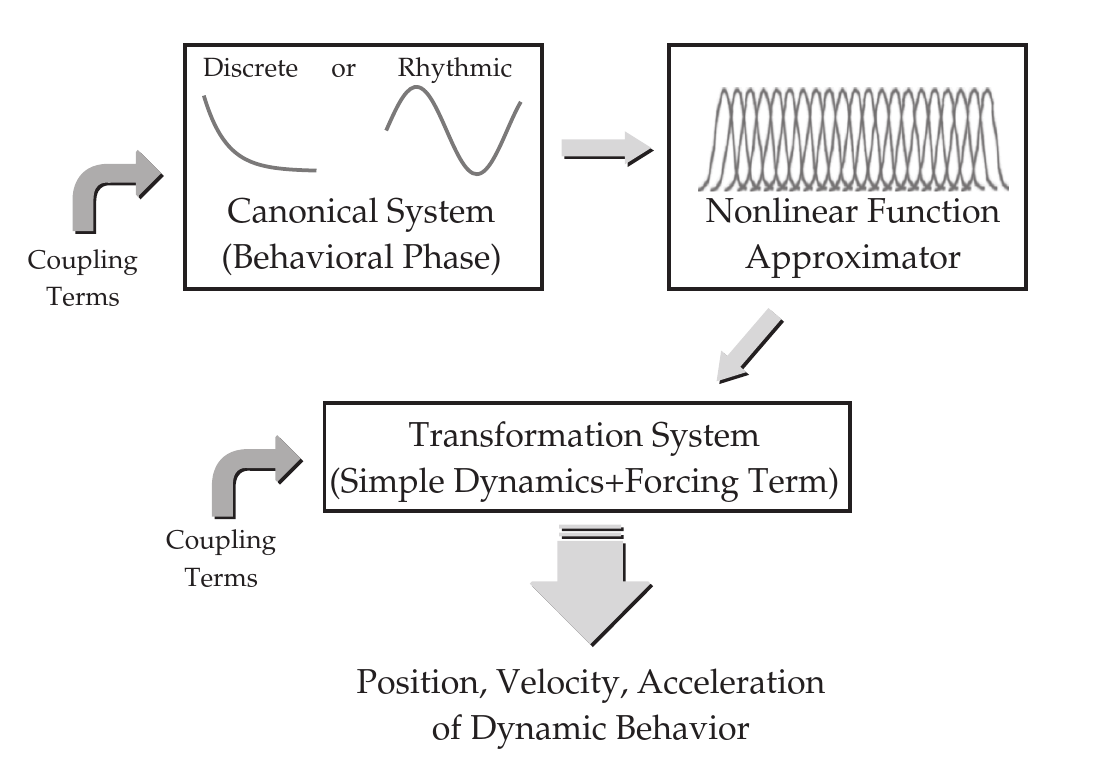
\includegraphics[width=\textwidth]{images/dmp.png}
%	\caption{Dynamic Movement Primitive framework}
%	\label{fig:DMP framework}
%\end{figure}


\par Figure 1 taken from \cite{ijspeert2013dynamical} show complete DMP framework. 

\subsection{Learning the Attractor Dynamics from Observed Behavior}
\par Learning attractor dynamics implies learning the parameters in equations 1,2,3,4 and 5. Above system presented in \cite{ijspeert2013dynamical} is linear in the weights $w_{i}$. So variety of learning algorithms can be used. \cite{ijspeert2013dynamical} uses locally weighted regression to learn the weights. Desired behavior that should be exhibited by the system is presented as a tuple ($y_{demo}(t)$, $\dot{y}_{demo}(t)$, $\ddot{y}_{demo}(t)$) representing position, velocity and acceleration respectively where $t = [1,2,3,4,....,p]$. Parameter $g$ is goal hence, $g = y_{demo}(t = p)$ and $y_{0} = y_{demo}(t = 0)$. Parameter $\tau$ is temporal scaling factor which needs to adjusted for achieving desired time scaling in the motion. In order to use LWR for estimating $w_{i}$, equation (1) can be rearranged to generate function approximation problem as ,
\begin{equation}
f = \tau\dot{z} - \alpha_{z}(\beta_{z}(g - y) - z)
\end{equation}
Inserting the information from the demonstrated trajectory in the left-hand side of this equation, we obtain
\begin{equation}
f_{target} = \tau^{2}\ddot{y}_{demo} - \alpha_{z}(\beta_{z}(g - y_{demo}) - \tau\dot{y}_{demo})
\end{equation}
By using any of the regression techniques on data obtained by above equation, we can estimate unknown weight ($w_{i}$) parameters in equation (3). 




\subsection{Inverse Kinematics Solver and Trajectory Controller}

In order to execute the task-space trajectory generated by DMP framework, Cartesian velocities are needed to be converted to the joint velocities with the help of inverse kinematic solver. Robot arm used in the experiments (KUKA YouBot arm) has five degrees of freedom. Five degrees of freedom are not sufficient to carry out 6 degrees of freedom cartesian motion. Due to this design deficiency, manipulator is always in the singular configuration. It is well-known that when a manipulator is at-or is in the neighborhood of a singular configuration, severe restrictions may occur on its motion. To overcome this situation, \textit{weighted damped least square pseudo inverse method} for computing joint velocities was chosen. This method allows us to loose the constraints on individual degrees of freedom in task-space. Which allowed us to ignore velocity constraints on 3 rotational degrees of freedom. This is called user-defined accuracy method to control the manipulator. \cite{chiaverini1994review}
\\
The relation between joint space and task space velocity can be given by, 

\begin{equation}\label{theta_dot}
	v = J(\theta) \dot{\theta} 
\end{equation}

\begin{equation}
	\dot{\theta} = J(\theta)^{-1}  v
\end{equation} 
Where, \\
$J(\theta)$ is jacobian of manipulator, \\
$v$ is task space velocity vector, \\
$\dot{\theta}$ is joint space velocity vector. \\

When manipulator is near a singularity, sigma  large joint velocities may occur or degenerate directions may exist where end-effector velocity
is not feasible\cite{chiaverini1994review}. To overcome this situation, damped least square method can be used where a degraded solution is generated near the singularities proposed in \cite{wampler1986manipulator, nakamura1986inverse}.  

\begin{equation}
	J^{T}(\theta)v = (J^{T}(\theta)J(\theta) + \lambda ^{2}I)\dot{\theta}
\end{equation}

Where, \\
$\lambda > 0 $ is the damping factor, and \\
$I $ is identity matrix. \\

Solution to above problem can be given by, 
\begin{equation}\label{damped_least_sol}
	\dot{\theta} = (J^{T}(\theta)J(\theta) + \lambda^{2}I)^{-1}J^{T}(\theta)v
\end{equation} 

It should be noted that, if the value of $\lambda$ in eq. \ref{damped_least_sol} is set to 0, eq. \ref{damped_least_sol} reduces to eq. \ref{theta_dot}.

The effect of value of lambda on joint velocities can be analyzed in detail by singular value decomposition of the Jacobian matrix and that is, 

\begin{equation}
	J = \sum_{i=1}^{6}\sigma_{i}u_{i}\textbf{v}_{i}^{T}
\end{equation} 

Using singular value decomposition, equation \ref{damped_least_sol} can be rewritten as,

\begin{equation}
\dot{\theta} = \sum_{i=1}^{6}\frac{\sigma_{i}}{\sigma_{i}^{2} + \lambda^{2} }\sigma_{i}u_{i}\textbf{v}_{i}^{T}v
\end{equation} 

It can be observed in above equation that if $\sigma >> \lambda$, then $\lambda$ has practically no effect on joint velocities. But if $\sigma$ is close to zero, then the joint velocities are greatly affected by value of $\lambda$.  

Since the arm has only five degrees of freedom, it is always in singular configuration and hence it is not possible to execute the 6 degrees of motion at all the time instances. This situation can be overcome by ignoring motion in 3 rotational degrees of freedom with the help of the method called \textit{weighted damped least square pseudo inverse}. In this method, 	
\section{Setup}


\section{Experimental Design}
